In this sprint we focused on the 'Cars' project from last year's multi-project.
The main purpose of the sprint was to get an understanding of the project, while making it usable by eliminating bugs and implementing missing features.

Cars is a small game, in which the user controls a car, moving from left to right on a three-lane road.
The user must use voice input, based on pitch, to move the car up and down in order to dodge obstacles on the road and in the end manoeuvre the car into a garage.
A screenshot from the Cars app can be seen in \cref{fig:cars_screenshot}.

\begin{figure}[h]
\centering
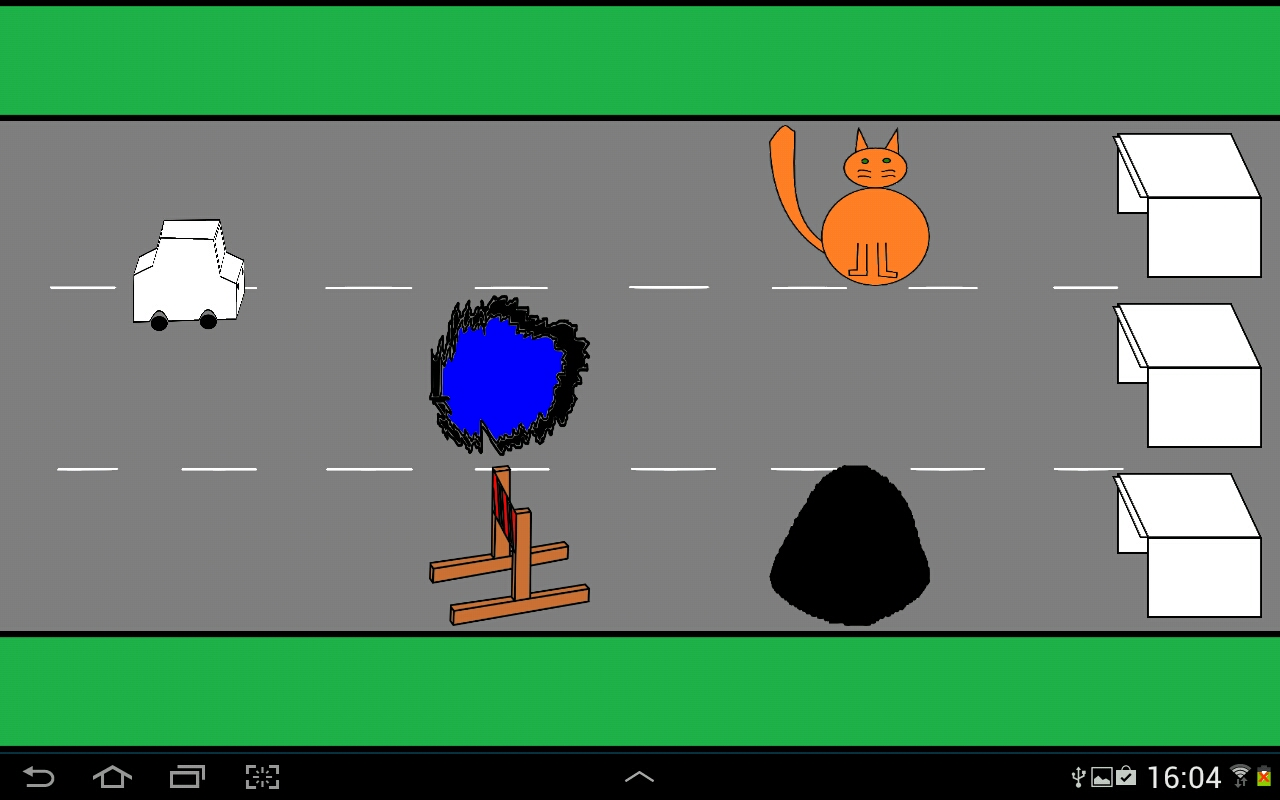
\includegraphics[width=.5\textwidth]{sprint1/cars_screenshot}
\caption{Screenshot from the 'Cars' app.}
\label{fig:cars_screenshot}
\end{figure}

Sound input is an important element of Cars, as it is used to control the car.
It was also a part of the game which did not work properly.
The movements of the car did not correctly correspond to the voice input, seemingly causing the car to move at random, no matter what kind of pitch was used.

Using voice input based on pitch was an original requirement of the Cars project, worked out between the Cars group and the stakeholders.
Its intention was to solve a particular problem concerning some autists, not being able to control their pitch during speech.
Based on its importance and that it does not work, this would be a natural major focus point during the first sprint.

However, we will argue that there are two overall problems with trying to improve the already existing Cars project.
Firstly we will argue that it is very difficult to obtain frequency from sound input.
Secondly we will argue that it would be easier to completely reboot the Cars project, with new framework and structure, rather than continuing on the existing code and structure.

We will instead argue for using volume instead of pitch, after confirming its validity with the stakeholders.
Additionally we will propose a structure, based on the KiloBolt framework.